\subsubsection{Ajustes del algoritmo basados en pruebas unitarias 1}
    Recopilando los datos obtenidos en algunas de las pruebas
        unitarias realizadas hasta el momento de realizaci\'on de estas
        mismas, se aplicaron algunos cambios al programa,
        principalmente enfocados a mejorar cada una de sus
        funciones y que sea mucho m\'as f\'acil en cuanto a la calidad
        del algoritmo.
        \vskip 0.5cm
    Los cambios que han sido aplicados hasta el momento
        corresponden a los siguientes elementos que conforman el
        programa:
        \vskip 0.5cm
    %figura
    \begin{figure}[htbp]
        \centering
        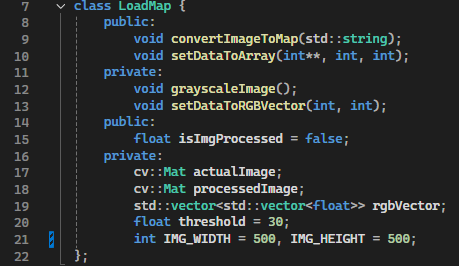
\includegraphics[width=0.5\textwidth]{./images/Pruebas/simulador/image045.png}
        \caption{Implementaci\'on del LoadMap}
        \label{fig:Pruebaunitaria2}
    \end{figure}
    Implementaci\'on de la clase LoadMap: A pesar de que se
        pueda configurar un espacio en el lienzo por medio del
        dibujo, muchas veces al querar colocar un croquis o un mapa
        de determinado espacio, dibujar a mano con el rat\'on resulta
        poco conveniente, por lo que se implement\'o la clase
        LoadMap, la cual hace uso de la librer\'ia OpenCV,
        transformando una imagen en un dibujo en el lienzo del
        programa al inicializarse este \'ultimo. Esto se puede ver en
        la Figura \ref{fig:Pruebaunitaria2}.
        \vskip 0.5cm
    %figura
    \begin{figure}[htbp]
        \centering
        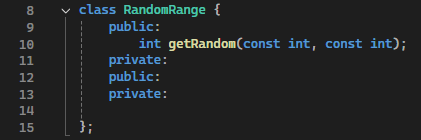
\includegraphics[width=0.5\textwidth]{./images/Pruebas/simulador/image046.png}
        \caption{Clase RandomRange}
        \label{fig:Pruebaunitaria3}
    \end{figure}
    Clase RandomRange: Al realizarse las primeras pruebas
        unitarias en el software, fue obtenido como resultado que es
        poco conveniente usar la funcion rand() debido a que tiende
        a ser mucho m\'as lenta que otras implementaciones, adem\'as
        de que su aleatoriedad no es la mejor y adem\'as, no es
        multihilo, lo que impide que si en el futuro el algoritmo se
        quiere paralelizar, esto dificulte la implementaci\'on denumero randoms que sean thread safe. Esto se puede ver en
        la Figura \ref{fig:Pruebaunitaria3}.
        \vskip 0.5cm
